\chapter{Concepts}
\section{Introduction}
The \emph{Jupiter} system is a collaboration system that supports shared documents, shared tools, and, optionally, live audio/video communication. It was developed by \emph{Xerox}. It is conceptually a collaborative windowing toolkit. The low-level communication facilities are based on operational transformation.

The operational transformation algorithm employed in the \emph{Jupiter} system is derived from \emph{dOPT}. A centralized architecture and thus the reduction to point-to-point connections makes the algorithm significantly simpler than other operational transformation algorithms. The basic \emph{Jupiter} algorithm is only suitable for two sites. However, it was shown in \cite{jupiter95} and in greater detail in \cite{netedit:thesis} how to use several point-to-point connections to build a tree-structured $n$-site algorithm (see figure \ref{fig:concepts.nway}).

\begin{figure}[htb]
 \centering
 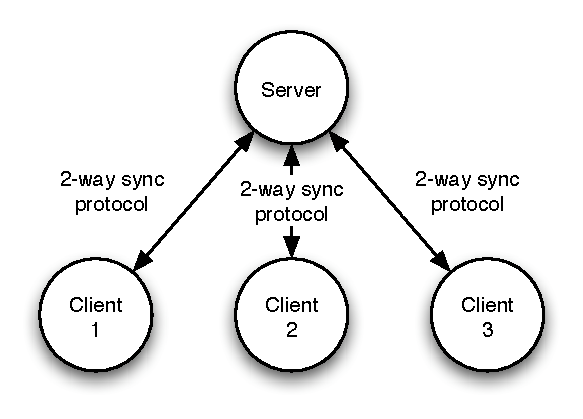
\includegraphics[width=7cm,height=4.89cm]{../../images/concepts_nway.eps}
 \caption{multiple 2-way sync to achieve n-way sync}
 \label{fig:concepts.nway}
\end{figure}

\section{Jupiter Algorithm}
A collaborative editing application requires that local operations are immediately applied to the local document and then sent in a request (that includes a vector time) to other sites. This can result in two or more operations that are executed concurrently. The general tool for handling these conflicting (i.e. concurrent) requests is a transformation function, called $xform$ in \cite{jupiter95}.

$$ xform(c,s)=\{c',s'\} $$

This transformation function takes two operations, $c$ from the client and $s$ from the server, and returns two transformed operations $c'$ and $s'$. The operations $c'$ and $s'$ have the property that if the client applies $c$ followed by $s'$, and the server applies $s$ followed by $c'$, both client and server wind up in the same final state (see figure \ref{fig:concepts.basic}). This property is also known as transformation property 1 (TP1):

$$ c s' \equiv s c' $$

Conceptually, the $xform$ function is a combined inclusion transformation (IT) that returns $\{IT(c,s),IT(s,c)\}$. The parameters $c$ and $s$ must originate from the same document state. This is a necessary precondition of inclusion transformation. If this precondition is violated, the result of the transformation is not guaranteed to be correct.

\begin{figure}[htb]
 \centering
 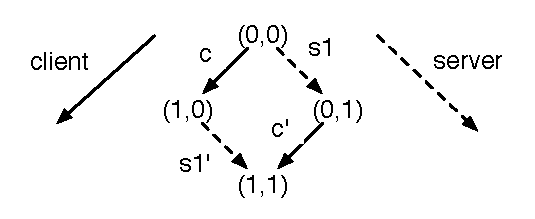
\includegraphics[width=6.85cm,height=2.5cm]{../../images/concepts_jupiter1.eps}
 \caption{basic transformation situation in jupiter}
 \label{fig:concepts.basic}
\end{figure}


\subsection{State Space Graph}
As we have seen, it is helpful to show the two dimensional state space that both client and server pass through as they process requests (see figure \ref{fig:concepts.statespace}). Each state is labelled with the number of processed requests from both client and server to that point. For instance if the client is in the state $(2,3)$, it has generated and processed two requests of its own, and has received and processed three from the server. The client and server requests are displayed on different axis in the state space graph.

\begin{figure}[htb]
 \centering
 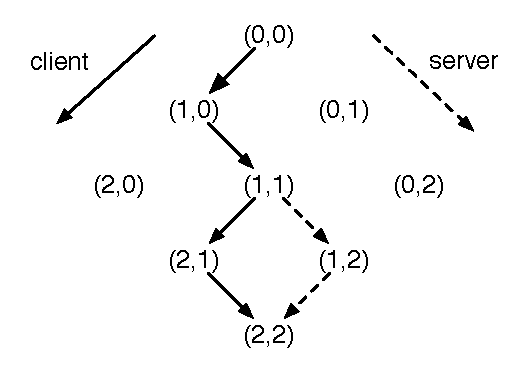
\includegraphics[width=6.63cm,height=4.5cm]{../../images/concepts_statespace.eps}
 \caption{two dimensional state space example}
 \label{fig:concepts.statespace}
\end{figure}

If there is a conflict, the paths will diverge, as shown in figure \ref{fig:concepts.statespace}. The client and server moved to the state $(1,1)$ together by first processing a client request, and then a server request. At that point, the client and server processed different requests (concurrently), moving to state $(2,1)$ and $(1,2)$ respectively. They each received and processed the other's message using the transformation function to move to state $(2,2)$.

The algorithm labels each request with the state the sender was in just before the message was generated (state vector). The recipient uses these labels to insert the request at the correct position into his state space. If the request does not start from the current state of the recipient, there is a conflict (concurrent request). Two concurrent requests have to be transformed, but they can only be transformed directly when they were generated from the same document state.

If client and server diverge by more than one step in the state space graph, the transformation function cannot be applied directly. Let us consider the state space in figure \ref{fig:concepts.statespace2}. The client has executed $c$ and receives the conflicting request $s1$ from the server. It uses the transformation function to compute $s1'$ to get to the state $(1,1)$. The server then generates $s2$ from the state $(0,1)$, indicating that it still has not processed $c$. What should the client do now? It cannot use the transformation function directly because $c$ and $s2$ were not generated from the same document state.

\begin{figure}[htb]
 \centering
 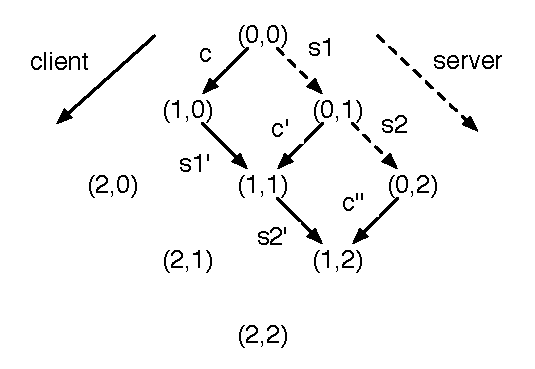
\includegraphics[width=6.71cm,height=4.5cm]{../../images/concepts_statespace2.eps}
 \caption{client and server diverging by more than one path step}
 \label{fig:concepts.statespace2}
\end{figure}

The solution to this situation is as follows. When the client computes $s1'$ it must also remember $c'$. This represents a hypothetical request that the client could have generated to move from the state $(0,1)$ to $(1,1)$. When $s2$ arrives, the client can use $c'$ to compute $c''$. It executes $s2'$ to get to the state $(1,2)$. If the server has processed the client's message, it will be in the state $(1,2)$ as well. If not, its next request will originate from $(0,3)$, so the client saves $c''$ just in case.

The algorithm guarantees that if the transformation function satisfies TP1, then no matter how far the client and server diverge in state space, when they do reach the same state (and they do, unless requests get lost), they will have equivalent states (so convergence is achieved).



\subsection{Extending Jupiter to N-Way Communication}
We have discussed how a single two-way connection works in \emph{Jupiter}. We will now extend this systems to support $n$ clients using multiple two-way connections. The figure \ref{fig:concepts.nway-details} shows the basic setup for three clients. Each client talks only to the server over a standard previously discussed two-way connection. On the server, there is one so-called client proxy per client. This client proxy conceptually is just the server side algorithm. 

\begin{figure}[htb]
 \centering
 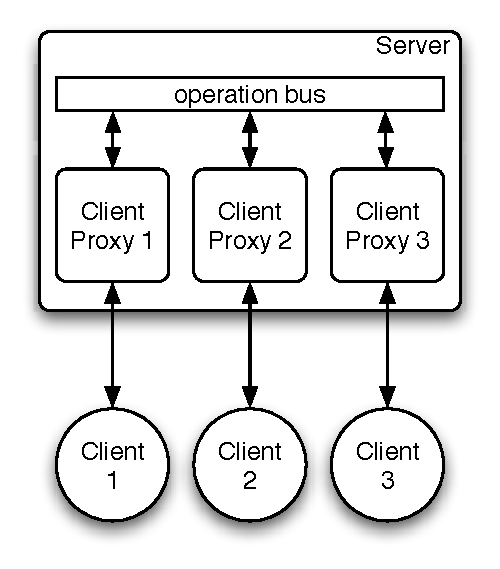
\includegraphics[width=5.23cm,height=6cm]{../../images/concepts_nway-details.eps}
 \caption{n-way synchronization using central server}
 \label{fig:concepts.nway-details}
\end{figure}

When a client, let us say client 1, sends a request to the server, the corresponding client proxy algorithm transforms the request against any concurrent requests the server already sent to this client but that were not acknowledged by it. Client proxy 1 then dispatches the transformed operation to all other client proxies. The other client proxies (client proxy 2 and 3) get this operation and insert it into their algorithm as local operation (resulting in a new request). The resulting request is then sent to the client 2 and 3 respectively. 

\textbf{Note:} One thing must be taken care of in the implementation. Only one request may be processed by the server at any time. That is, the processing of requests from clients must be serialized. Otherwise, the algorithm will not work correctly.

\paragraph{n-way example:} In order to better understand how the n-way synchronization work, we examine a simple example. In the following 4 figures, the bottom two state graphs represent two clients, the top two state graphs represent the server, or more exactly the client proxy algorithms on the server. 

In the first step, both clients generate a request concurrently and send it to the server (see figure \ref{fig:concepts.nway-example-1}). Then the request from client 1 arrives at the server earlier than the request from client 2 and is therefore processed first (see figure \ref{fig:concepts.nway-example-2}). In the next step, the request from client 2 is processed by the server (see figure \ref{fig:concepts.nway-example-3}). In the last step both clients receive the transformed request from their corresponding client proxy on the server side (see figure \ref{fig:concepts.nway-example-4}). They insert the requests at the right positions in their state space, doing transformations as necessary (client 2 has to transform the incoming message, client 1 not).

\begin{figure}[H]
 \centering
 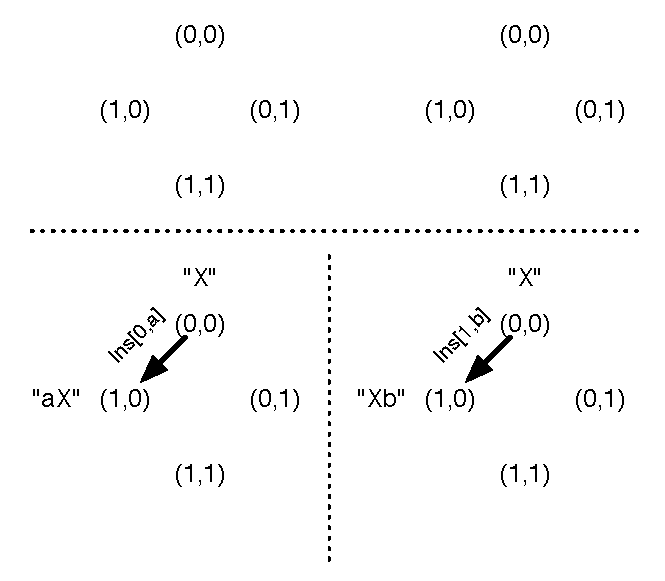
\includegraphics[width=10.0cm,height=7.54cm]{../../images/concepts_nway-example-1.eps}
 \caption{n-way example (step 1)}
 \label{fig:concepts.nway-example-1}
\end{figure}

\begin{figure}[H]
 \centering
 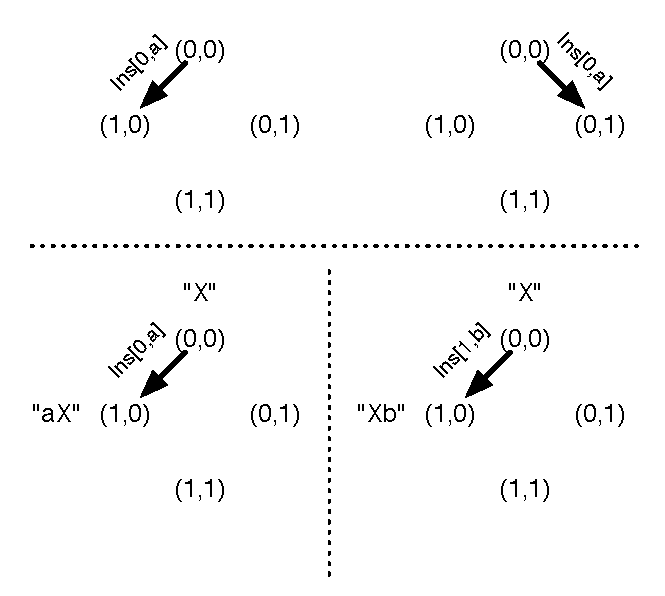
\includegraphics[width=10.0cm,height=7.74cm]{../../images/concepts_nway-example-2.eps}
 \caption{n-way example (step 2)}
 \label{fig:concepts.nway-example-2}
\end{figure}

\begin{figure}[H]
 \centering
 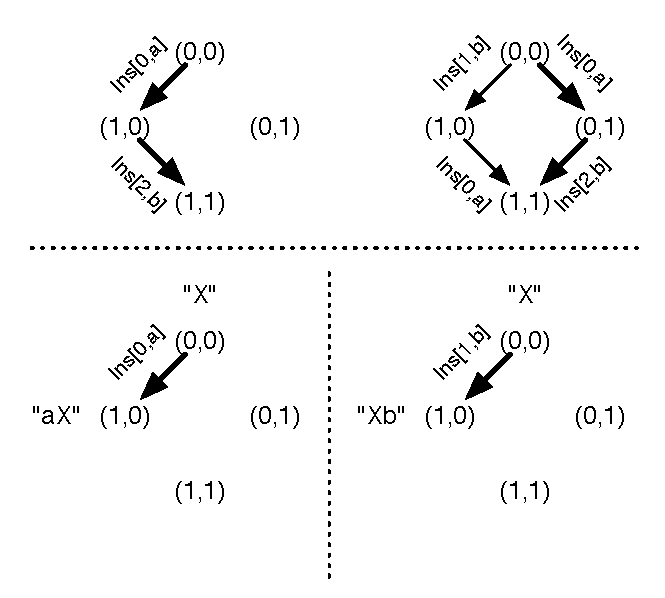
\includegraphics[width=10.0cm,height=7.77cm]{../../images/concepts_nway-example-3.eps}
 \caption{n-way example (step 3)}
 \label{fig:concepts.nway-example-3}
\end{figure}

\begin{figure}[H]
 \centering
 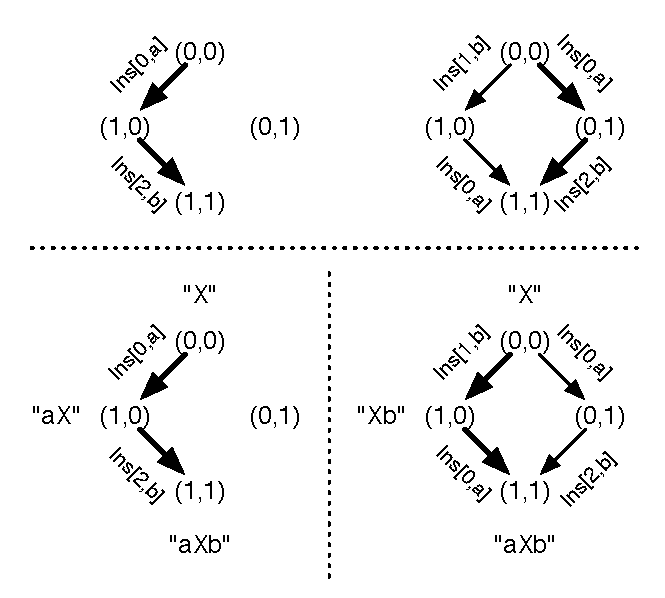
\includegraphics[width=10.0cm,height=7.77cm]{../../images/concepts_nway-example-4.eps}
 \caption{n-way example (step 4)}
 \label{fig:concepts.nway-example-4}
\end{figure}


\section{Undo/Redo}
In the preceeding sections, we have presented the basic transformation algorithm. In this section we will show how undo/redo of local operations can be achieved in a real-time collaborative editor. This introduces a whole set of new problems that necessitate additions and modifications to the transformation algorithm. The concepts of this undo solution are partially taken from \cite{ressel99} (\emph{adOPTed} algorithm) but are significantly extended and adapted to the \emph{Jupiter} algorithm.

\subsection{Problems of Local Group Undo}
Global group undo is not much different from common single-user undo schemes. It can be implemented by executing the inverse operation for each user operation to be undone. The operation to be undone is the globally last operation that was executed. Global undo always leads to a former application state. In contrast, local group undo (undoing the last operation from the local user) is more complex, because in most cases it does not lead to a former application state.

\paragraph{Example 1:} 
\label{example1}
Suppose the initial document state is 'm'. Now user $X$ executes the operation \texttt{Ins[1,s]} to insert the character 's' at position 1 of the document. Then user $Y$ executes \texttt{Ins[1,a]} to insert the character 'a' at position 1 resulting in a document state 'mas'. Now user $X$ decides to undo his last insertion operation. What has to be done? The naive, but incorrect approach would just execute \texttt{Del[1,s]}, i.e. the inverse to \texttt{Ins[1,s]}. However, the current character at position 1 is not 's' but 'a'. The situation is depicted in figure \ref{fig:concepts.naiveundo}.

\begin{figure}[htb]
 \centering
 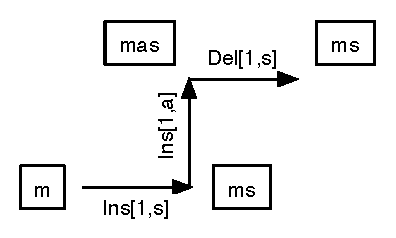
\includegraphics[width=6.13cm,height=3.45cm]{../../images/concepts_naiveundo.eps}
 \caption{incorrect naive approach to local group undo}
 \label{fig:concepts.naiveundo}
\end{figure}

Obviously, just executing the inverse of the last local operation cannot achieve the correct result. In addition, there are more situations were local group undo methods can fail. One characteristic example is the following problem, which is called \emph{order puzzle}.

\paragraph{Example 2:}
\label{example2}
Suppose we start with a document containing 'ab'. Now user 'X' first deletes 'a' by executing \texttt{Del[0,a]}. Afterwards user $Y$ deletes 'b' by issuing the operation \texttt{Del[0,b]}. This will leave the document empty. Now both users undo their operations. The expected application state should be 'ab' afterwards, because undoing all operations should not modify the original application state. Unfortunately, a naive undo solution could yield the wrong state 'ba'. The solution to the order puzzle will be presented in a later section (see section \ref{sect:concepts.order-puzzle-solution}).

\subsection{Transformation-Based Local Group Undo}
Let us return to the example 1. Suppose we want to undo the last operation after an operation from another participant has already been executed. For correctness of local group undo, we require that the effect of the undo request does not depend on other users' requests. Therefore, we may safely assume, that we issued the undo operation immediately after the execution of the operation to be undone. Then the appropriate transformations can be applied to gain the operation that has to be executed in the present state. 

In example 1, we insert the inverse operation \texttt{Del[1,s]} immediately after the operation. The procedure of inserting the inverse operation is called \emph{mirroring}. In the next step, the inverse operation \texttt{Del[1,s]} is transformed against the operation \texttt{Ins[1,a]} from user $Y$, which results in the correct operation \texttt{Del[2,s]}. See figure \ref{fig:concepts.undobytransformation}.

\begin{figure}[htb]
 \centering
 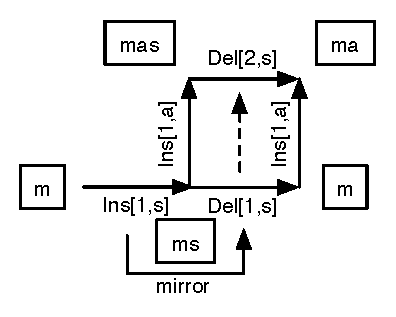
\includegraphics[width=6.13cm,height=4.79cm]{../../images/concepts_undobytransformation.eps}
 \caption{local undo by applying transformations}
 \label{fig:concepts.undobytransformation}
\end{figure}

Unfortunately, the computation of requests in the interaction model by transformation and by mirroring is not sufficient to solve the \emph{order puzzle} in example 2.

\paragraph{Example 3:} 
\label{example3}
Suppose both users $X$ and $Y$ simultaneously delete the single character 'b' (see figure \ref{fig:concepts.basicfold}). The corresponding transformation rule transforms both operations to \texttt{Noop} operations (no operation, operation without any effect on the document state), since deleting the same character twice is impossible. Now suppose, user $Y$ wants to undo his operation \texttt{Del[0,b]}. We know this can be achieved by applying the mirror operator, producing the operation \texttt{Ins[0,b]}. Now, how can the missing operations be computed? By just applying the transformation rule, the operations would just be copied without modification, e.g., another \texttt{Noop} operation would lead from state 'b' to the end state 'b' (in the upper right corner). However, this violates the principle of correctness, namely that a set of do-undo pairs like \texttt{Del[0,b]} and \texttt{Ins[0,b]} should have no effect on other users' operations. If this were to be satisfied, the resulting state should be empty, like when executing user X's operation \texttt{Del[0,b]} only. 

\begin{figure}[htb]
 \centering
 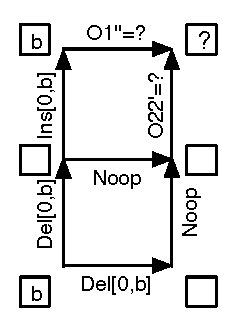
\includegraphics[width=3.45cm,height=4.97cm]{../../images/concepts_basicfold.eps}
 \caption{application of mirror and fold operators}
 \label{fig:concepts.basicfold}
\end{figure}


\subsection{Fold Operator}
To solve the puzzle in example 3, we observe that all parallel lines connected by do-undo pairs should actually contain congruent requests and states. Here in the example $O_{1}''$ should be \texttt{Del[0,b]}, and the resulting state should be empty, like the operation and the state at the bottom of the diagram (see figure \ref{fig:concepts.basicfold}).

We denote the copying of a request from the beginning of a do-undo pair - or more general a set of possibly nested do-undo pairs - to the end of the do-undo pair as \emph{folding}. This illustrates the fact that we might actually fold the interaction model - here along the straight line defined by the horizontal \texttt{Noop} request in the center - so that both lines come to lie above each other. 

To complete the interaction model we demand that $O_{22}'$ will be computed by mirroring the operation \texttt{Noop} (in figure \ref{fig:concepts.basicfold} at the bottom right). The resulting interaction model with all mirror and fold operators applied is displayed in figure \ref{fig:concepts.basicfold-solution}.

\begin{figure}[htb]
 \centering
 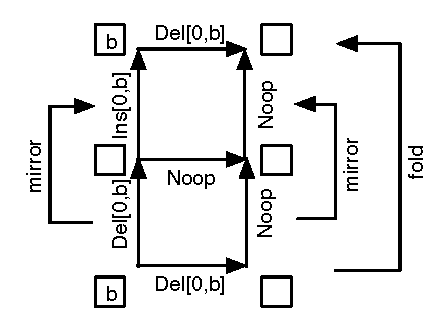
\includegraphics[width=6.99cm,height=4.97cm]{../../images/concepts_basicfold-solution.eps}
 \caption{application of mirror and fold operators}
 \label{fig:concepts.basicfold-solution}
\end{figure}


\subsection{Solution to the Order Puzzle}
\label{sect:concepts.order-puzzle-solution}
The solution to the order puzzle in example 2 can be computed with the same operators, mirror and fold. The desired result is shown in figure \ref{fig:concepts.orderpuzzle}.

\begin{figure}[htb]
 \centering
 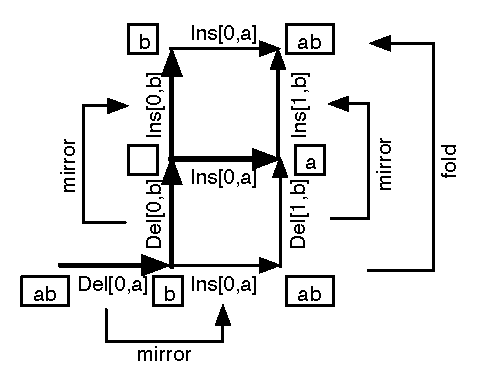
\includegraphics[width=7.55cm,height=5.96cm]{../../images/concepts_orderpuzzle.eps}
 \caption{Solution to the Order Puzzle}
 \label{fig:concepts.orderpuzzle}
\end{figure}


\subsection{Additional Problems in n-Way Situation}
Unfortunately, there exists another problem in the n-way situation that do not exist in the 2-way situation. To illustrate the problem and the solution we introduce another example.

\paragraph{Example 4:} First, user $X$ generates the request \texttt{Del[0,b]} from the initial document state 'b'. Then, he undoes that change immediately (generating the mirror request \texttt{Ins[0,b]}). User $Y$ generates the request \texttt{Del[0,b]} concurrently to the two requests from user $X$ (see figure \ref{fig:concepts.transformation-history-1}). In figure \ref{fig:concepts.transformation-history-2} the first request from user $X$ is processed by the server and then by the user $Y$. Nothing unusual happens in this situation. Then the request from user $Y$ is processed by the server, resulting in a \texttt{Noop} operation (see figure \ref{fig:concepts.transformation-history-3}).

The next step (see figure \ref{fig:concepts.transformation-history-4}) reveals the problem. The \texttt{Noop} operation is inserted into the state space of user $X$. Now we need to calculate operation $O_{x}$. Because the \texttt{Noop} operation is between a do-undo pair (mirror), $O_{x}$ must be calculated by folding the state space graph, that is by putting the dashed operation $O_{x}$ from the bottom to the top line. The problem is, we do not know what this operation was, so we cannot apply the fold operator.

In figure \ref{fig:concepts.transformation-history-5} we see a similar problem on the server-side. Here, the undo request from user $X$ has arrived at the server and is inserted into the state space graph at the correct position (from $(0,1)$ to $(0,2)$). Because we have a do-undo pair (mirror) on the bottom line, we must have a mirror operation on the second line too according to our transformation rules. In order to calculate $O_{y}$ we need to know the operation marked with three question marks first. This operation can be calculated by transforming \texttt{Del[0,b]} against $O_{x}$. Once again, it is the operation $O_{x}$ that is missing.

So how do we find out $O_{x}$? The answer lies in the fact that the \texttt{Noop} request resulted from a transformation, so $O_{x}$ was known by the client proxy of user $Y$ (\texttt{Del[0,b]}). If we save the transformation history of an operation, we can use these previous forms of an operation to successfully apply mirror and fold operators and thus solve the problem presented in this example.

\begin{figure}[H]
 \centering
 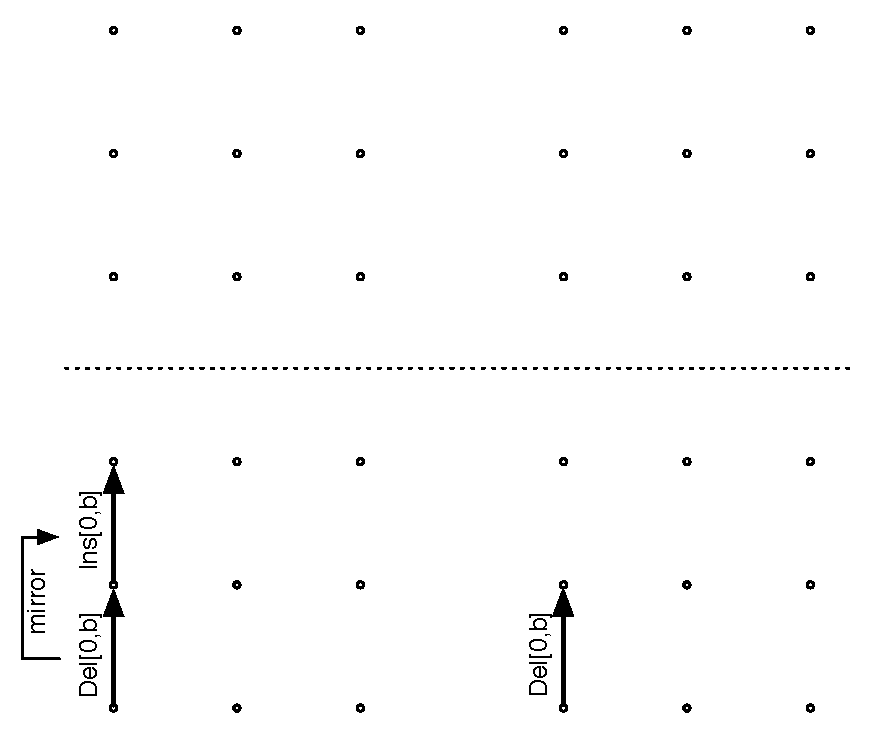
\includegraphics[width=10cm,height=8.36cm]{../../images/concepts_transformation-history-1.eps}
 \caption{n-way undo problem (step 1)}
 \label{fig:concepts.transformation-history-1}
\end{figure}

\begin{figure}[H]
 \centering
 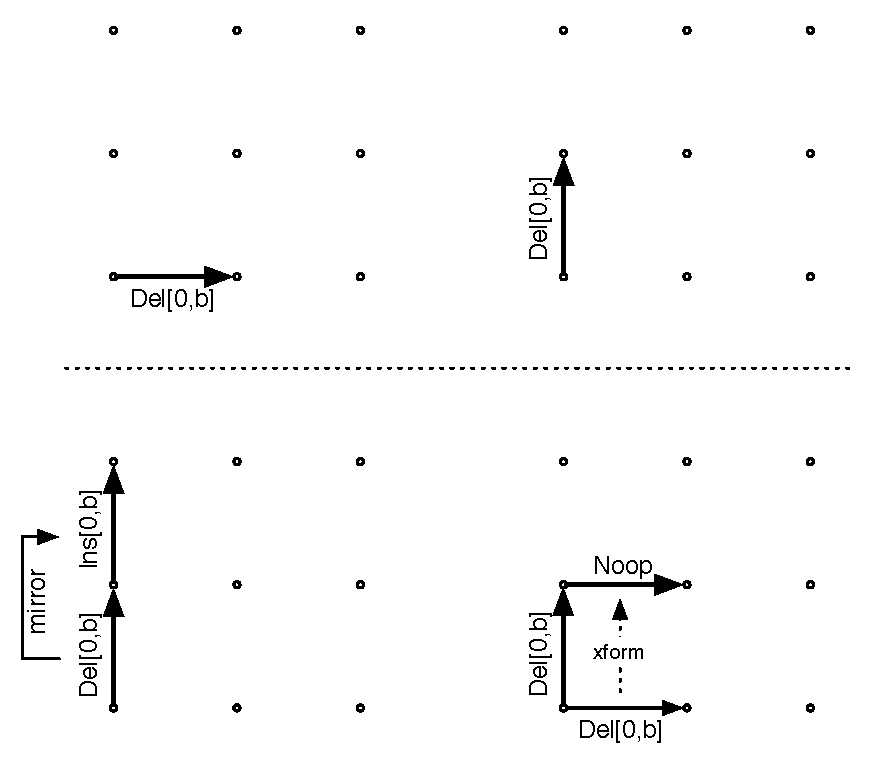
\includegraphics[width=10cm,height=8.69cm]{../../images/concepts_transformation-history-2.eps}
 \caption{n-way undo problem (step 2)}
 \label{fig:concepts.transformation-history-2}
\end{figure}

\begin{figure}[H]
 \centering
 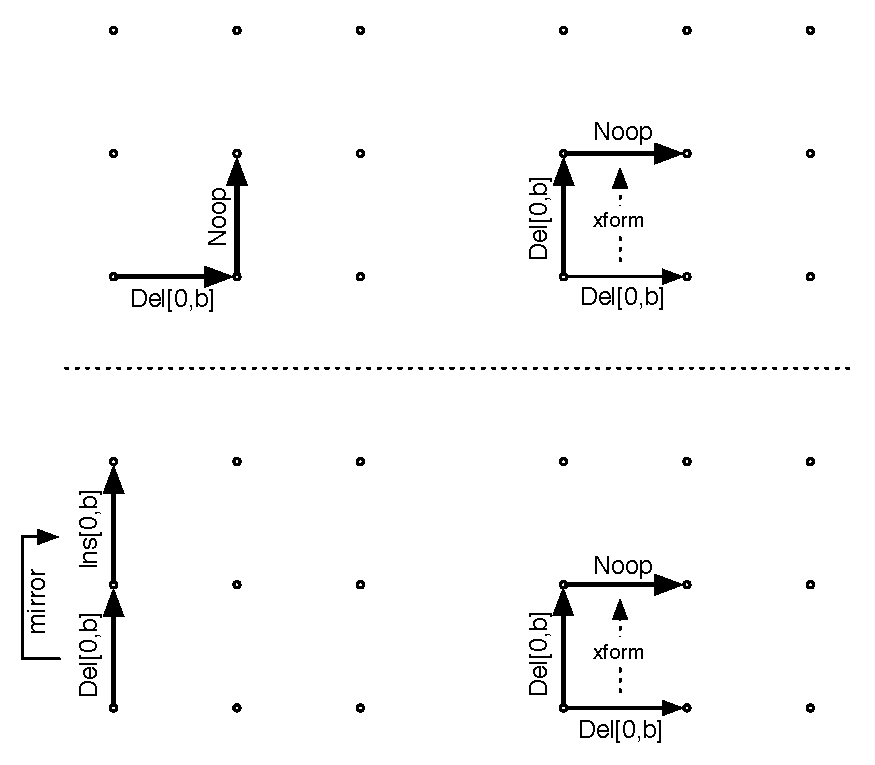
\includegraphics[width=10cm,height=8.69cm]{../../images/concepts_transformation-history-3.eps}
 \caption{n-way undo problem (step 3)}
 \label{fig:concepts.transformation-history-3}
\end{figure}

\begin{figure}[H]
 \centering
 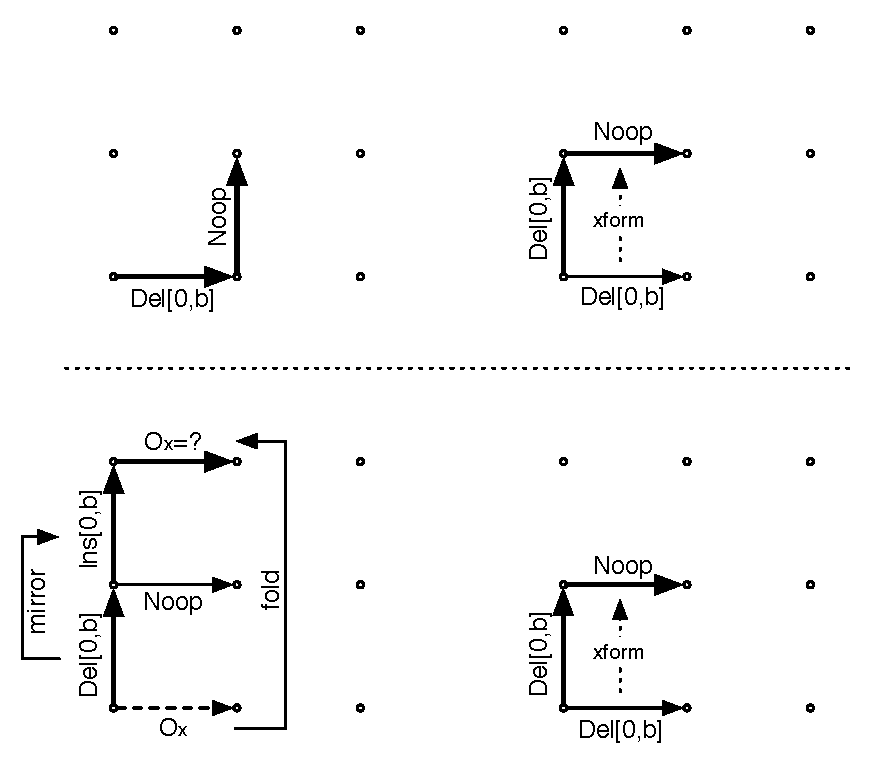
\includegraphics[width=10cm,height=8.69cm]{../../images/concepts_transformation-history-4.eps}
 \caption{n-way undo problem (step 4)}
 \label{fig:concepts.transformation-history-4}
\end{figure}

\begin{figure}[H]
 \centering
 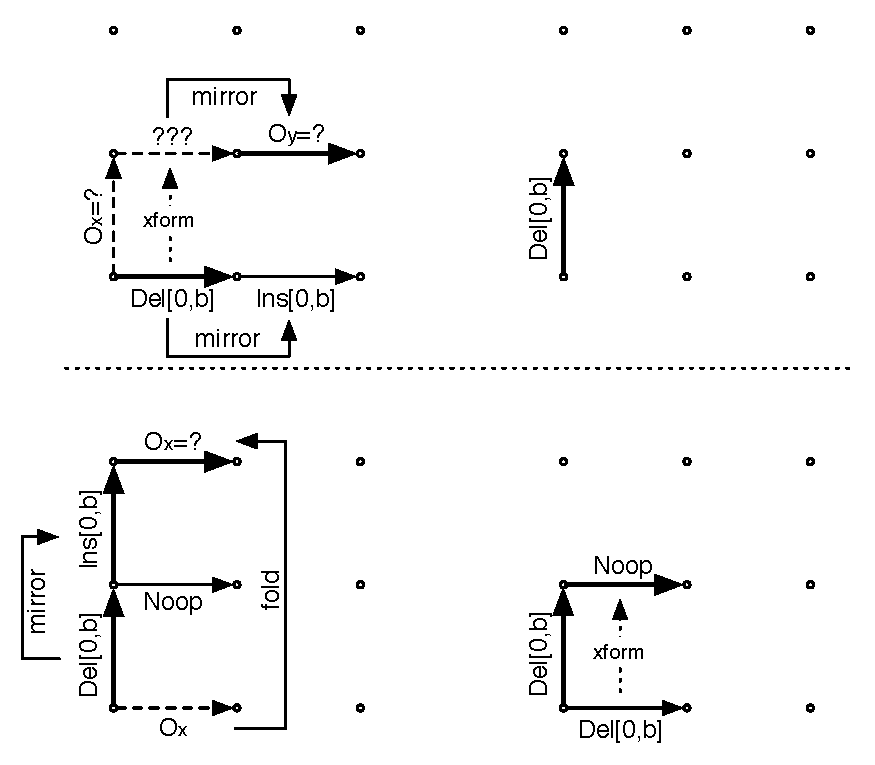
\includegraphics[width=10cm,height=8.69cm]{../../images/concepts_transformation-history-5.eps}
 \caption{n-way undo problem (step 5)}
 \label{fig:concepts.transformation-history-5}
\end{figure}


\subsection{Redo}
The integration of a redo operation, as far as we know, has never been considered before in the area of operational transformation algorithms. However, it turned out to be rather straightforward to implement a redo feature. A redo can only be done, if the last operation from a user has been an undo or there are only undo-redo pairs between the current state and an undo operation. A do operation between the current state and an undo operation effectively disables the redo functionality (this is the normal behavior in any modern text processing application).

\begin{figure}[htb]
 \centering
 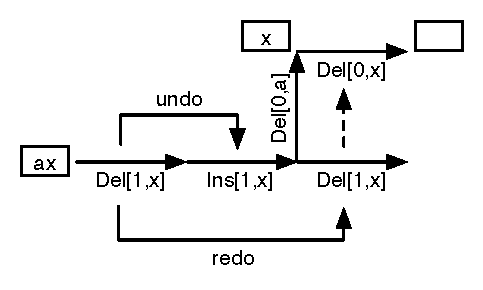
\includegraphics[width=7.62cm,height=4.34cm]{../../images/concepts_redo.eps}
 \caption{Redo Operation}
 \label{fig:concepts.redo}
\end{figure}

In figure \ref{fig:concepts.redo} we see how a redo is inserted into the state space. First, the last operation from this user must be a undo (or there are only undo-redo pairs between the current state and an undo operation). This is clearly the case in this example. We then copy the corresponding do operation to the current column in the state space on the same line as the original operation (see arrow labeled redo). Then, we have to transform this copied operation to the current state, so that it can be applied. 


\section{GOTO Transformation Functions}
\label{GOTO Transformation Functions}

\subsection{Overview}
The GOTO (generic operation transformation optimized) transformation functions are designed to work with strings as well as characters. The advantage is that less transformations have to be done when a string is inserted into a text. To understand the exigence of transformation functions see \emph{Report Evaluation Algorithms}.

The inclusion transformation functions are used to include the effect of a given operation B into another operation A. The transformed operation A' is returned. To transform an operation means to adapt position and text of the operation. In the majority of cases this is a very simple process. But sometimes it is necessary to extract a text fragment or to split up an operation into two parts. For more details about splitting operations see \ref{Split_Operation}.

All possible transformation \emph{cases} with two insert/delete operations are depicted in figure \ref{Transformation Overview} and explained in the following sections:
\begin{figure}[H]
\centering
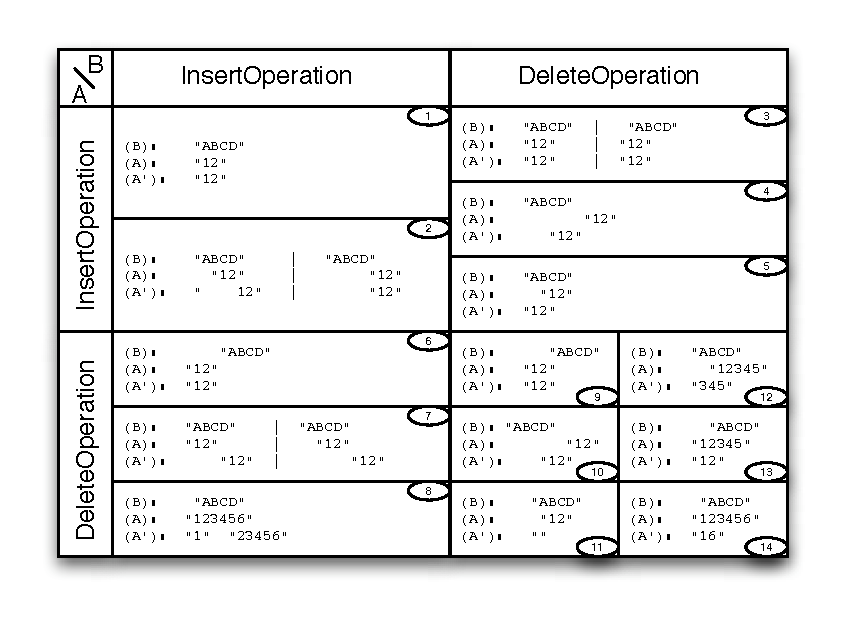
\includegraphics[height=9.98cm,width=13.75cm]{../../images/algo-impl/transform_overview.eps}
\caption{Transformation Overview}
\label{Transformation Overview}
\end{figure}

\subsection{Insert/Insert}
\begin{itemize}
\item \textbf{Case 1:}
Operation A starts before or at the same position as operation B. Sometimes a special handling is necessary. See \emph{Special Case} in section \ref{Special_Case} for detailed information about that.
\item \textbf{Case 2:}
Operation A starts inside or after operation B. Index of operation A' must be increased by the length of the text of operation B.
\item \textbf{Special case:}
\label{Special_Case}
It can happen that two insert operations (for example \texttt{Ins(0,'a')} and \texttt{Ins(0,'b')}) have the same position. How should the correct transformation look like (does the insertion of 'a' have to be before or after 'b')? This is an undecidable problem. Therefore some extra rules must be defined. The first approach to solve this problem is by preferring the operation with the lower ascii value. With this method the final text would be 'ab'. The following figure demonstrates that this solution can violate the user's intention:
\begin{figure}[H]
\centering
%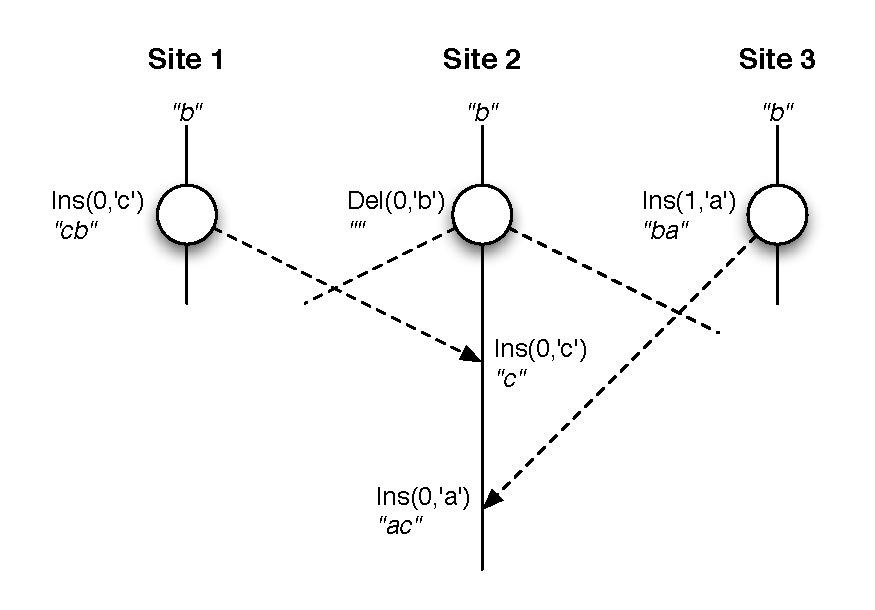
\includegraphics[height=9.77cm,width=14.25cm]{../../images/algo-impl/transform_ins_ins_charpos.eps}
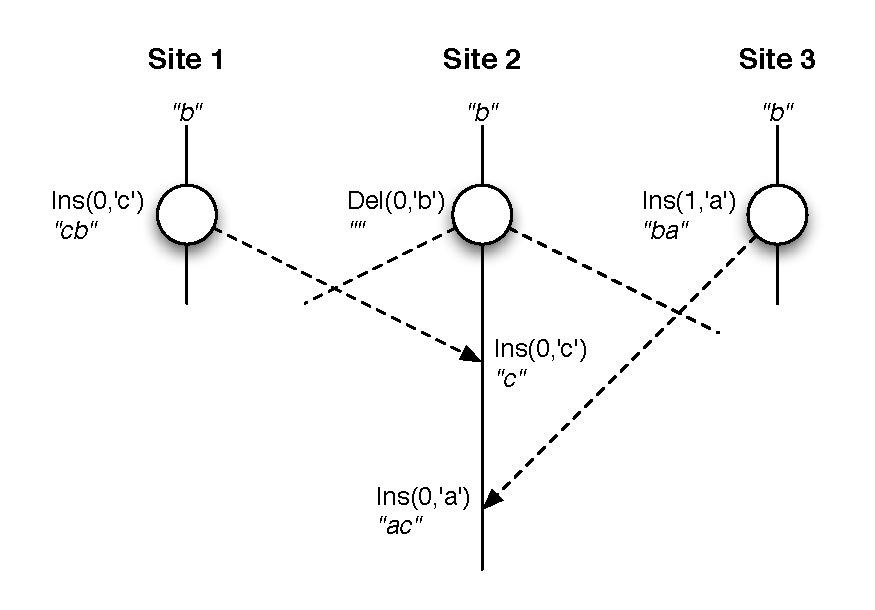
\includegraphics[height=4.63cm,width=7.12cm]{../../images/algo-impl/transform_ins_ins_charpos.eps}
\caption{Transformation based on character code}
\label{Transformation based on character code}
\end{figure}
The scenario depicted in figure \ref{Transformation based on character code} demonstrates an editing session with 3 users (sites). Each site generates a request concurrently. For simplicity only the process flow at site 2 is shown. The initial document state is 'b'. After applying the own operation (\texttt{Del(0,'b')}) the document becomes empty. Then the two other operations arrive. First the operation \texttt{Ins(0,'c')} from site 1 and then \texttt{Ins(1,'a')} from site 3, which will be transformed into \texttt{Ins(0,'a')}, because the delete operation has an effect on it. The two operations (\texttt{Ins(0,'a')} from site 3 and \texttt{Ins(0,'c')}) from site 1 must be transformed and the resulting document state becomes 'ac', which violates the user intentions.

The second approach works with some extra information. If an operation has been generated, the original position is saved too. Adapted to the scenario in figure \ref{Transformation based on character code} the insert operation of site 1 would look like \texttt{Ins(0,'a',0)}. Similar to the insert operation of site 1 the insert operation of site 3 looks like \texttt{Ins(1,'b',1)}. The added third parameter represents the original position. At the beginning the position and the original position have the same value. The difference of the two positions is shown after a transfomation. Unlike the position (first parameter) the original position will never be transformed/changed and remains the same for the livetime of the operation.

Considering the second approach, the site 1 sends the request \texttt{Ins(0,'c',0)} to site 2. After site 2 received the request, site 3 sends the request \texttt{Ins(1,'a',1)}. On site 2 this request will first be transformed against \texttt{Del(0,'b')} into \texttt{Ins(0,'a',1)}. This is necessary because while site 3 was generating the request, site 2 deleted the character \texttt{b}. After this transformation the new request has to be transformed with the request from site 1. This transformation would look like \texttt{transform( Ins(0,'a',1), Ins(0,'c',0) )} which means that the effect from the operation \texttt{Ins(0,'c',0)}) will be included into operation \texttt{Ins(0,'a',1)}. Now the problem is the same as before, but with the extra information it can be solved. After detecting that the two operations have the same position the transformation function compares the original positions. With this solution the 'c' will be inserted before the 'a' and the user intention is preserved.

Unfortunately figure \ref{Transformation based on character code} shows that even with using original positions in the transformation function, problems can occur:
\begin{figure}[H]
\centering
%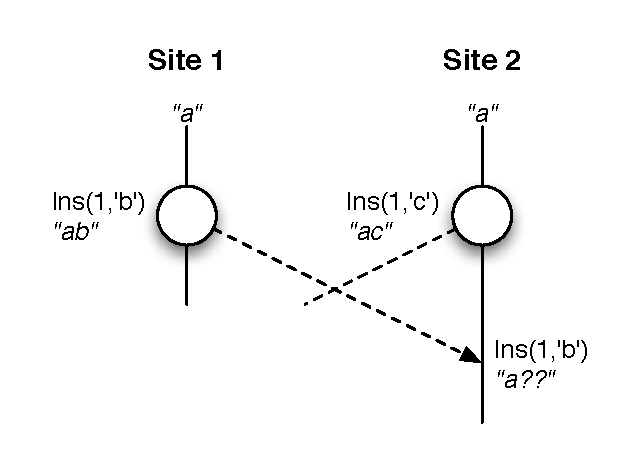
\includegraphics[height=7.26cm,width=10.26cm]{../../images/algo-impl/transform_ins_ins_origpos.eps}
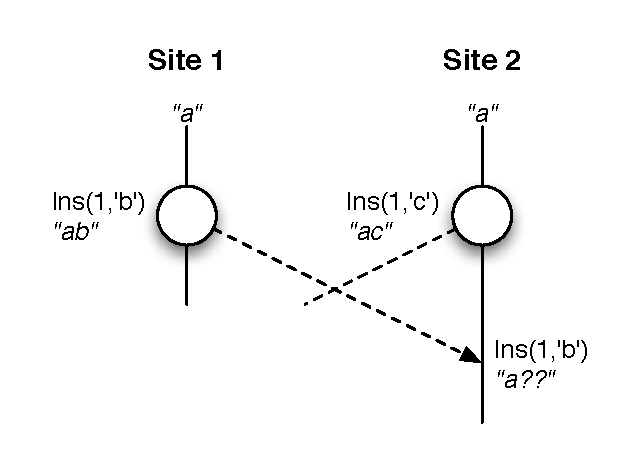
\includegraphics[height=3.63cm,width=5.13cm]{../../images/algo-impl/transform_ins_ins_origpos.eps}
\caption{Transformation based on equal original positions}
\label{Transformation based on equal original positions}
\end{figure}
At the same time each site generates an insert operation with the same position. The insert operation from site 1 looks like \texttt{Ins(1,'b',1)} and the operation from site 2 is \texttt{Ins(1,'c',1)}. When site 2 receives the request from site 1 the operations have to be tranformed (\texttt{transform( Ins(1,'b',1) , Ins(1,'c',1) )}). The transformation function will detect that the two operations have the same position and will check the original positions. Unfortunately the original positions have the same values. Therefore the approach to solve this problem by using original positions will fail too.

This problem can only be eliminated by privileging one operation. But which operation should be preferred? And how to guarantee that on all sites this will be the same operation? One possible solution would be to use the site id's (e.g. site 1 is always privileged against site 2 and site 3, site 2 is only privileged against site 3). When using this transformation function with the \emph{Jupiter} algorithm, the operation which has been issued by the server side is always privileged (client/server flag).

\item \textbf{The concept of last synchronization point (LSP)}
Again we consider the situation where to insert operation are to be transformed and both have the same positions. The comparison of the original positions works quite well as shown above. But it has shortcomings. What if the two operations do not relate on the same context and document state, respectively? Though the comparison of the original positions can still take place, it is a weak comparison because the user's intention may get lost as shown in the example depicted in the following figure:

\begin{figure}[H]
\centering
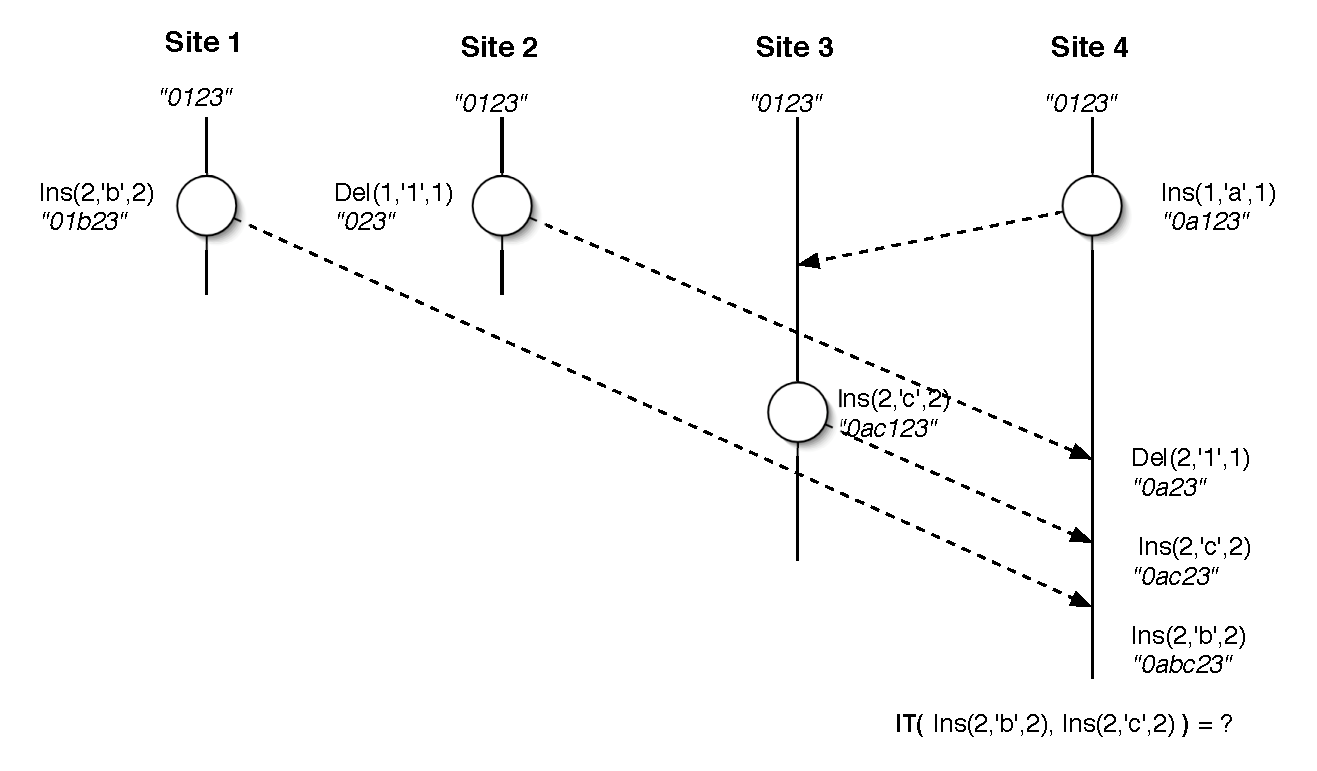
\includegraphics[height=3.69in,width=6.42in]{../../images/algo-impl/transform_ins_ins_lsp.eps}
\caption{Shortcoming of comparison with original positions}
\label{Shortcoming of comparison with original positions}
\end{figure}

Only site 4 is considered. When all operations have arrived, the last transformation to be done includes the two insert operations. Both are equivalent in that they have the same positions as well as the same original positions. The remarkable thing is that though the two original positions are equal, they do not relate on the same document state. Operation $Ins(2,'c',2)$ from site 3 was generated after the operation from site 4 had been received. It is clear that the user's intentions of site 3 and 1 are violated in that user 1 inserted 'b' after '1' and user 3 inserted 'c' before '1', but in the final document state the 'b' is placed before 'c'. Here the comparison of the original positions fails. We need a more advanced concept. 

Therefore we introduce the concept of "last synchronization point" (LSP), analogously adapted to our implementation of \emph{Jupiter}. It is taken from paper "Preserving Operation Effects Relation in Group Editors", Du Li and Rui Li. The idea comes right into play at the situation described above. When the two original positions need to be compared, it should first be ensured that both operations and original positions, respectively, rely on the same document state. If this happens, they can savely be compared and in case of equality the client/server flag included. If they do not relate on the same document state, we need to find a last synchronization point where the two operations can correctly be compared. In the example above, this would be achieved as follows. When the two insert operations are compared, it is detected that they cannot be compared as is. Therefore, the first operation from site 4 would be excluded from  operation $Ins(2,'c',2)$, which in fact is the first one at site 3. With this exclusion, we arrive at the same document state for both operations and thus we can compare them correctly. Operation $Ins(2,'b',2)$ would be transformed so that 'b' gets inserted after 'c', which was the user's implicit but actual intention.

Recapitulating, we would like to implement this concept to improve the system's ability to preserve the user's intention also in the most complex situations. Yet we do not know if the LSP concept can be implemented at all in our system. This feature is left open as future  work.
\end{itemize}

\subsection{Insert/Delete}
\begin{itemize}
\item \textbf{Case 3:}
Operation A starts before or at the same position as operation B. Nothing has to be transformed.
\item \textbf{Case 4:}
Operation A starts after operation B. Index of operation A' must be reduced by the length of the text of operation B.
\item \textbf{Case 5:}
Operation A starts inside operation B. Index of operation A' must be the index of operation B.
\end{itemize}

\subsection{Delete/Insert}
\label{Delete_Insert}
\begin{itemize}
\item \textbf{Case 6:}
Operation A is completly before operation B. Nothing has to be transformed.
\item \textbf{Case 7:}
Operation A starts before or at the same position as operation B. Index of operation A' must be increased by the length of the text of operation B.
\item \textbf{Case 8:}
Operation B is in the range of operation A. Operation A' must be splitted into two delete operations. For more details about the split operation see \ref{Split_Operation}.
\end{itemize}

\subsection{Delete/Delete}
\begin{itemize}
\item \textbf{Case 9:}
Operation A is completely before operation B. Nothing has to be transformed.
\item \textbf{Case 10:}
Operation A starts at the end or after operation B. Index of operation A' must be reduced by the length of the text of operation B.
\item \textbf{Case 11:}
Operation A and operation B are overlapping. Operation B starts before or at the same position as operation A and ends after or at the same position as operation A. Content of operation A has already been deleted by operation B. Therefore, nothing has to be deleted anymore by operation A. A' is called a noop (no-operation).
\item \textbf{Case 12:}
Operation A and operation B are overlapping. Operation B starts before or at the same position as operation A and ends before operation A. The overlapping part of the two operations has been deleted by operation B. Operation A' has to delete only the remaining text (text after the overlapping text of the two operations).
\item \textbf{Case 13:}
Operation A and operation B are overlapping. Operation B starts after operation A and ends after or at the same position as operation A. The overlapping part of the two operations has been deleted by operation B. Operation A' has to delete the remaining text (text before the overlapping text of the two operations).
\item \textbf{Case 14:}
Operation A and operation B are overlapping. Operation B is fully inside operation A. The overlapping part of the two operations has been deleted by operation B. Operation A' has to delete the remaining text (text before and after the overlapping text of the two operations).
\end{itemize}
